%\addcontentsline{toc}{chapter}{Development Process}
\chapter{Design}

%You should concentrate on the more important aspects of the design. It is essential that an overview is presented before going into detail. As well as describing the design adopted it must also explain what other designs were considered and why they were rejected.

%The design should describe what you expected to do, and might also explain areas that you had to revise after some investigation.

%Typically, for an object-oriented design, the discussion will focus on the choice of objects and classes and the allocation of methods to classes. The use made of reusable components should be described and their source referenced. Particularly important decisions concerning data structures usually affect the architecture of a system and so should be described here.

%How much material you include on detailed design and implementation will depend very much on the nature of the project. It should not be padded out. Think about the significant aspects of your system. For example, describe the design of the user interface if it is a critical aspect of your system, or provide detail about methods and data structures that are not trivial. Do not spend time on long lists of trivial items and repetitive descriptions. If in doubt about what is appropriate, speak to your supervisor.
 
%You should also identify any support tools that you used. You should discuss your choice of implementation tools - programming language, compilers, database management system, program development environment, etc.

%Some example sub-sections may be as follows, but the specific sections are for you to define. 

\section{Overall Architecture}

\section{Language Choice}
My language of choice for this project was Go\cite{GOLANG}
Also known as Golang, it is statically typed, compiled, concurrent and  garbage collected and is heavily inspired by C for the general syntax, Limbo for it's use of Communicating Sequential Processes (CSP)\cite{HOARE-CSP} and Python for its emphasis on readability and an all inclusive standard library.
It is relatively modern, only released to the public in 2009, and was created to solve some of the problems experienced with the languages used at Google, namely C\verb!++!, Python and Java.
I began to learn it, through the Golang Challenge\cite{GOLANG-CHALLENGE},  during my industrial year after experiencing some of these problems with python myself.

The creators of the language are all well respected in the world of computing.
Rob Pike is known for Plan 9 and UTF8. 
Robert Griesemer for the Java hotspot VM
Ken Thompson for Unix, Plan 9 and B, the predecessor to C.
Their combined hatred of the complexity and compile times of C\verb!++! where the catalyst for Go's development.
They also saw it as an opportunity to improve upon the aspects of C that have been most problematic over the years including:

\begin{itemize*}
	\item Optional braces around if statements (The cause of apples GOTO fail bug\cite{GOTOFAIL}).
	\item Pointer arithmetic.
	\item Confusing side effects of post/pre increment and decrement. Go only allows the post version and only as a standalone expression.
	\item GOTO statements that can jump anywhere at any time.
    \item Overloaded return values used to indicate errors.
\end{itemize*}

The language also avoided style wars as it came with a tool, gofmt, that formats code 'the right way'.
This is just one of the ways in which Go is extremely opinionated.
Others include:
\begin{itemize*}
	\item Unused imports and variables are a compile time error.
    \item Variables names should be generally be short. The longer they are in scope the longer and more descriptive the name should be.
    \item The use of interface composition over polymorphism, generics and inheritance.
    \item One loop construct, the for loop. Use with a break statement to create a while or until loop.
\end{itemize*}

It also comes with a simple built in testing framework that encourages tests right from the start and a documentation generator emphasising that.


It also doesn't hurt that Go has been found that to be a great language to build components traditionally done with C, including things as complicated as a kernel subsystem\cite{GONET}.

Concurrency after moores law, cores increasing faster than ghz.

While this is the language I decided to go with in the end I did consider others.
The candidate list included C, C\verb!++!, Python and OCaml.

\subsection{C}
C is a fast, low level, general purpose compiled language that is extremely powerful.
Unfortunately this power comes at a cost.
Historically the readability of C code is low which means that maintaining and extending code is hard.
This would not a huge problem if I was only creating the project for the dissertation but I hope to continue development after submission.

I considered it as a candidate as many shells have already been written using it proving it is a suitable choice.
This could be considered both an advantage, the abundance of prior art, and a disadvantage, less room to find innovative solutions.

While I have used some C in the past and have read the seminal book, K\&R C, I would not consider myself experienced in its use, especially with the more modern aspects like compiler directives and function annotations.
This could have led to problems around having to learn parts of such a complex language while developing a large project.
Even though I did not end up using this language I spent lots of time reading the source code for dash, bash and busybox which are all written in C, therefore using it  may have helped in my context switches. 

One thing I was worried about was the minimal standard library that C implementations provide.
I assumed that I would be required to spend valuable development time creating standard functions and data structures.
However during my research I discovered that libraries such as GLib and qLibc are commonly used and provide most, if not all, of the things I am used to in the StdLib of Python.

%XXX
Something to note is that I discovered a library, libmill\cite{LIBMILL}, which provides functions and macros for Go like CSP.

In conclusion the reasons I did not choose this as the implementation language was the verbosity of manual memory management and the aforementioned possibilities of bugs and lack of maintainability. 


\subsection{C++}


As with anything based in C, C\verb!++! may be considered the obvious step forward.
I have never used the language but have read the source code for a few projects written using it.
It has a fairly complete standard library and some of the memory management is abstracted behind constructor's and destructor's.
Despite this it is notoriously difficult and If the project where to use it it may be tied to one architecture and OS unless a lot of extra effort was put in.

\subsection{OCaml}
OCaml is a functional, garbage collected, compiled language.
It is a multi paradigm language that allows users to mix object oriented, imperative and functional styles.

I considered it as a candidate as it is often said that ML languages are superior to imperative ones at creating compilers and interpretors.
I chose it instead of other functional languages as it has recently been used to create some the high profile language Hack at Facebook.
As well as this it has been used for the Haxe language, the MirageOS unikernel and many code analysis tools.
These are all complex systems that show that the performance and the bulitin parsing tools are up to tasks well above the complexity of a simple interpretor.


I however had no experience at all with OCaml and very little with ML languages in general


\subsection{Python}



\section{Some detailed design}
The program is, at its core, a series of transformations that result in the initial text input being executed in various ways on the machine.

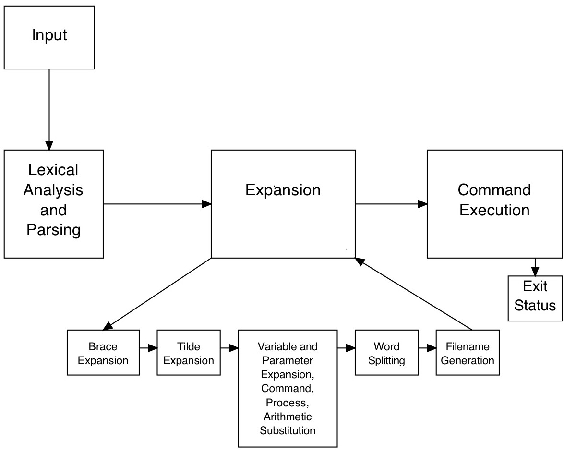
\includegraphics{bash-diagram.png}

\subsection{Even more detail}

\section{User Interface}

\section{Other relevant sections}